\documentclass{article}
\usepackage[utf8]{inputenc}
\usepackage{graphicx}
\usepackage{biblatex}

\addbibresource{references.bib}

\title{Radiatively-driven convection in a shallow ice-covered lake: 
temperature profiles dynamics, energy budget and mixing efficiency.
}
\author{}
\begin{document}

\maketitle

\section{Introduction}
The mechanisms of mixing the thermally stratified fluids and estimations of their efficiency remain the challenging problem in the theory of stratified turbulence during decades. For both mechanical and buoyancy-driven types of turbulent energy supply the gradient sharpening enhances the irreversible processes, and one of the key questions concerns the relationship between mixing (smoothing of spatial temperature distribution) and viscous dissipation. The quantitative description is traditionally based on exploring the energy budgets and, correspondingly, the conversions between different energy “reservoirs”: kinetic (KE), potential (PE) and internal (IE) energy. While the viscous dissipation is commonly identified by the rate of kinetic energy dissipation rate $\varepsilon$, the relevant measure of mechanical energy dissipation by turbulent mixing is questionable and still debated. Historically ~\cite{turner_buoyancy_1973,Lorenz1955}
%the ratio of $\varepsilon$ and KE production P was used as the first version of mixing efficiency. 
the turbulent buoyancy flux B was the first choice used as this measure. Correspondingly, the  mixing efficiency $\gamma$ was defined as $\gamma = B/(\varepsilon)$, or, equivalently by the flux Richardson number ~\cite{Ivey,Imberger, 1991}:   

\begin{equation}\label{eq:Ri}
Ri_f = B/(B+\varepsilon)
\end{equation}

Nowadays, however, it is widely recognized that B, being the indicator of reversible conversion between KE and PE, is not the proper direct measure of irreversible mixing.   


Instantaneous and local definitions ...

\section{Vendury 2016}

\begin{figure}
    \centering
    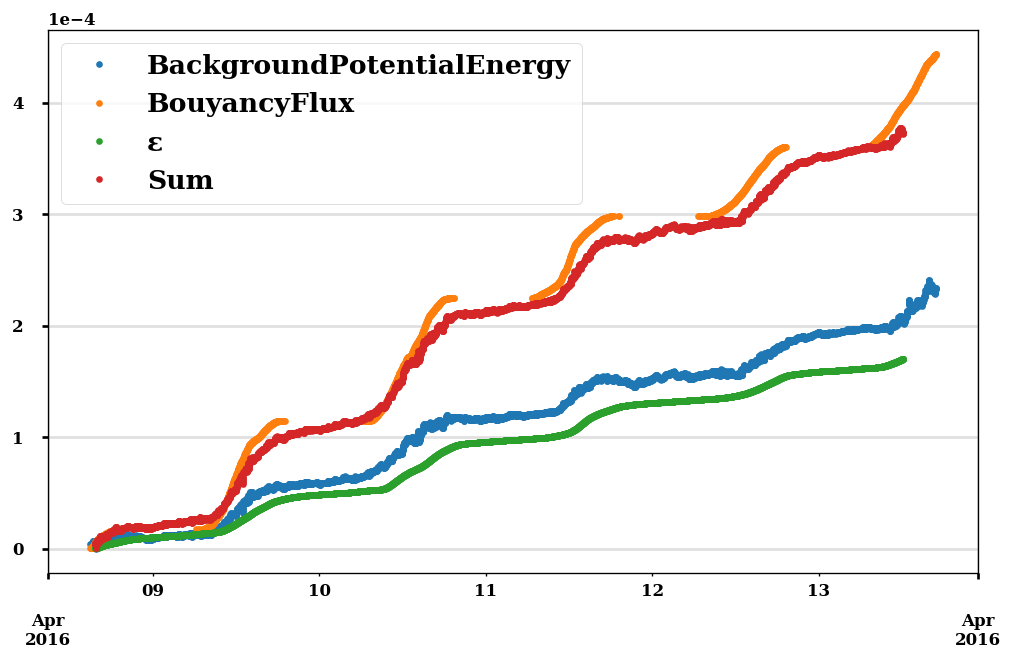
\includegraphics[width=\textwidth]{vend2016.png}
    \caption{The Sum line is a sum of $\varepsilon$ and BPE}
    \label{fig:my_label}
\end{figure}

\section{Vendury 2018}

\begin{figure}
    \centering
    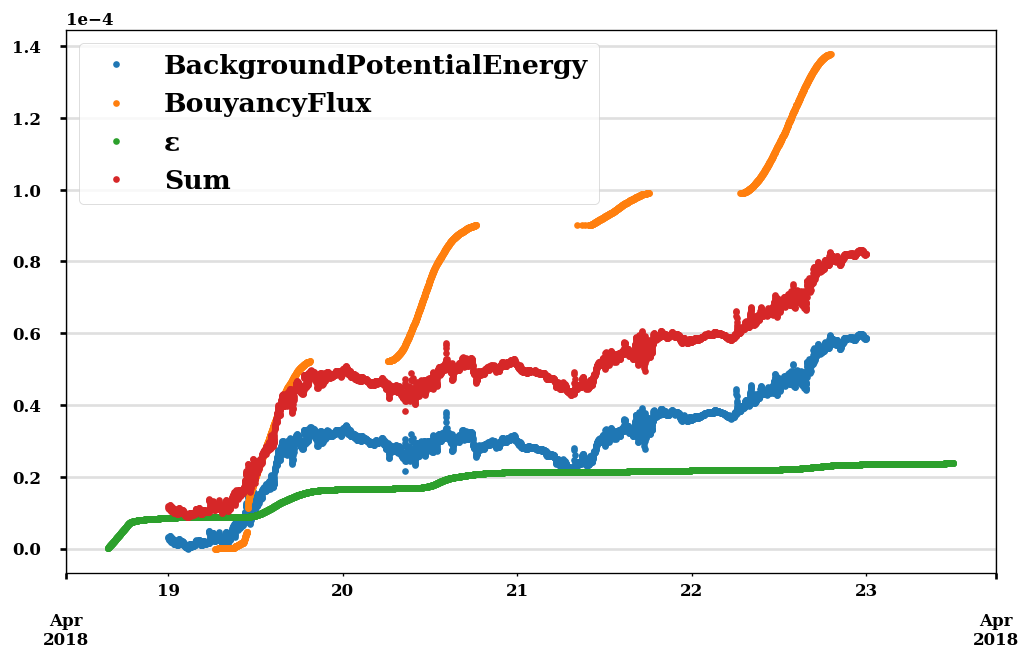
\includegraphics[width=\textwidth]{vend2018.png}
    \caption{Caption}
    \label{fig:vend2018}
\end{figure}

\printbibliography
\end{document}
